
% Problem Analysis and Goals
\section{Psychophysiological Framework}
To fully understand the role of psychophysiologic measurement in adaptive automation we will take a look at the theoretical frameworks behind it. However, providing a complete overview on this topic would be far too extensive for the scope of this thesis. Therefore, we will only give a short summary of the work done by Byrne and Parasuraman (1996).\\
The application of physiological measures in adaptive automation is built on the premise that there is indeed an ideal mental state for human operators in a given task environment and that any deviation from this state would be detectable in the measurement. 
This hypothesis is based on resource and capacity theories of information processing, which suggest that humans draw from a limited pool of resources whenever they process information \cite{Byrne1996}. Over the years, many researcher delivered evidence for a connection between this resource utilization and physiological measures of activation, therefore establishing the importance of psychophysiological measures in the field of adaptive automation.\\
%For instance, while both cognitive and compensatory effort were associated with physiological measures, psychological and physiological strain, arising from mental overload or underload, were detected in psychophysiological measurements. \\
However, psychophysiological measures perform a dual role in adaptive automation systems. First, there is the investigatory role, which is often referred to as the developmental approach. This approach is focused on using the information psychophysiological measures provide on the mechanisms underlying performance changes corresponding to changes in automation, and further the development of model-based and hybrid approaches \cite{Byrne1996}. The second role, is often characterized as the regulatory approach. Here, unique information about the human operator is gathered from psychophysiologic measurements. This information is then used as input to a hybrid adaptive logic, thus allowing for dynamic restructuring of the task environment. Although, this approach seems ideal to support the operation of an adaptive system due to its the immediate effect on the automated work environment, there may be years of effort and considerable maturation in technology required for it to be efficient in its application.  

\section{Psychophysiological Measures}
The identification of suitable psychophysiological measures plays a vital role to the success of an adaptive work environment. Considering the dual role framework of psychophysiology, there is a distinction to be made between the two applications in adaptive automation. Because the developmental approach is in alignment with the majority of applications in psychophysiological research, the often stated criteria of specificity, diagnosticity, and intrusiveness for selecting workload assessment techniques also hold for adaptive automation \cite{Byrne1996}. On the other hand, criteria for the regulatory role of psychophysiology in adaptive automation have to be more strict. As they become part of closed-loop systems operating in real-time their potential impact is far greater, and their effects more immediate compared to when used for developmental measures.  
In addition, the cost in terms of intrusiveness and technical requirements have to be weighed against the explanatory power of a certain measure. If the gain in predictive value does not offset the cost of implementation, a measure is not considered for applications outside of laboratory environment.\\
As the recent work is determined to employ the Empatica E4 wristband, we are limited to the measures that are provided by this platform. These measures are blood volume pulse (\gls{bvp}), skin response (\gls{gsr}), and surface temperature.

\section{Photoplethysmography}
Photoplethysmography \gls{ppg} is an optical measurement technique, used to detect blood volume changes in the microvascular bed of tissue \cite{Allan2007}. To work PPG only requires a few opto-electronic components. First, a light source is used to illuminate the tissue. Then a photodetector measures the variations in light intensity associated with changes in perfusion in the catchment area. 
The most common light sources in PPG produce wavelengths in the red or near infrared area. This specific part of the spectrum, also referred to as the optical water window, is chosen for its ability to pass through biological tissue with relative ease. Therefore, influences associated with light-tissue interactions are widely reduced and the measurement of blood flow or volume is facilitated at these wavelengths.
Even so, because the PPG is representing an average of all blood volume in the arteries, capillaries, and any other tissue through which the light has passed. The
PPG signal is dependent on the thickness and composition of the tissue beneath the sensor, as well as the position of the source in relation to the receiver of the infrared light \cite{Peper2007}.\\

\subsection{The PPG waveform: characteristics and analysis} 

The PPG waveform is comprised of two major components. The pulsatile component, often referred to as the "AC" component, possesses a fundamental frequency of approximately 1 Hz, and it represents the increased light attenuation associated with the increase in microvascular blood volume with each heartbeat \cite{Allan2007}. It is superimposed onto the much larger "DC" component, which relates to the tissue and the average blood volume contained in the observation area. Variations in the DC component are slower and caused by respiration, vasomotor activity and vasoconstrictor waves, as well as thermoregulation \cite{Allan2007}.\\ 

%[insert: ppg_raw.jpg, source: \cite{Allan2007}]
\begin{figure}[ht]
	\centering
  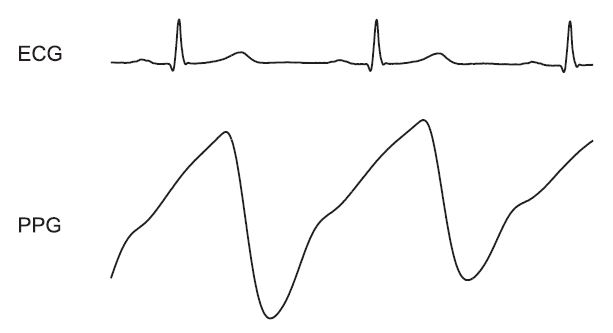
\includegraphics[width=0.7\textwidth, angle=0]{images/ppg_raw.jpg}
	\caption[PPG signal]{The PPG signal and the corresponding ECG. Displayed are the pulsatile AC component, which is super imposed on the much larger DC component. The PPG waveform represents light attenuation in relation to the blood volume in the tissue.}
	\label{ppg_pw}
\end{figure}

Its synchronization with the heart beat makes the AC pulse of the PPG waveform a valuable source of information on heart functions and condition. Based on the appearance of the AC pulse, two phases have been defined, reflecting its two most important properties. The first was labeled as the anacrotic phase and describes the rising edge of the pulse. This part of the waveform is primarily related to the systole. The second phase, shows the effects of diastole and wave reflections from the periphery of the vascular system. This phase is called catacrotic and can be observed in the successive falling edge of the pulse. In healthy subjects there usually is an observable dicrotic notch during this phase.
%[insert: ppg_pw.jpg, source: \cite{Allan2007}]
\begin{figure}[ht]
	\centering
  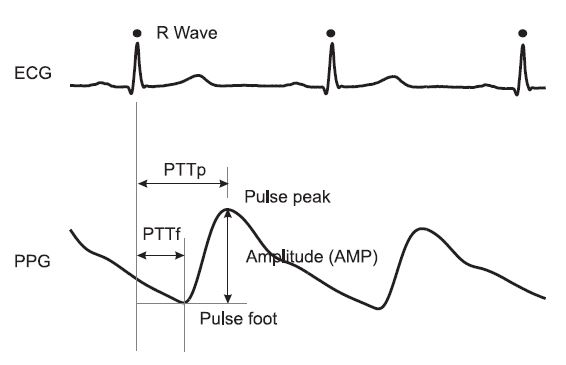
\includegraphics[width=0.7\textwidth, angle=0]{images/ppg_pw.jpg}
	\caption[PPG pulse characteristics]{Characteristics of the PPG pulse waveform in relation to the ECG.}
	\label{ppg_pw}
\end{figure}

In addition to this coarse classification, a number of key landmarks have been defined to facilitate the analysis of the waveform and the underlying physiology. Depicted in \ref{ppg_pw} are the three main features that are derived from a single pulse. The pulse transit time to the foot (\gls{pttf}), and the pulse transit time to the peak (\gls{pttp}) are defined as the time delays between a heartbeat, indicated by the R-wave of the \gls{ecg}, to the onset and the peak of the subsequent AC pulse.
The amplitude of a pulse is determined by the absolute value of the displacement between its base and its peak, which are marked by the aforementioned temporal features.\\
However, the scale of these characteristics, as well as the overall appearance of the waveform are still subject to change. It is believed that these changes are largely caused by reflection of the pulse wave and the tapering down of the arteries towards the periphery \cite{Allan2007}.\\
Another important consideration in the analysis of PPG signals is their susceptibility to movement related artifacts. Although, there are a number of different artifacts that could occur we will only inspect the ones relative to our application. As we employed the Empatica E4, a wrist worn device, to measure \gls{bvp} most of the artifacts are related to large movement of the arm and the wrist but also to small tremors in the hand or fingers. Additionally, extremes in physiological variation such as coughing and marked changes in the breathing pattern prove to be quite influential. Figure \ref{ppg_a} shows an illustration by Allan (2007) depicting the effects of movement related artifacts to one minute PPG recordings that were taken at the index finger.\\

%[insert: ppg_a.jpg, source: \cite{Allan2007}]
\begin{figure}[ht]
	\centering
  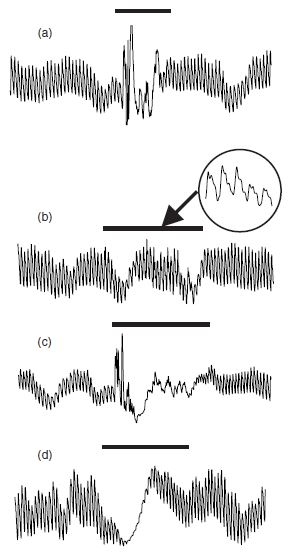
\includegraphics[width=0.5\textwidth, angle=0]{images/ppg_a.jpg}
	\caption[Types of measurement artifacts]{Examples of different types of measurement artifacts. All events were marked by black bars. (a) An episode of gross movement artifact of PPG probe cable tugging. (b) Hand or finger tremor. (c) a bout of coughing, and (d) marked changes in the breathing pattern (a deep gasp or yawn) }
	\label{ppg_a}
\end{figure}

This concludes the section on the general waveform morphology and the reasoning for its variations. Lastly, we will take a closer look at the features we derived from the PPG measurement, specifically heart rate, and heart rate variability.

\subsection{Heart Rate Variability}
Variations in the length of the intervals between consecutive heart beats are called heart rate variability (\gls{hrv}). Typically these inter beat intervals (\gls{ibi}s) are determined by calculating the distance between two subsequent R-peaks of an ECG signal. However, they can also be derived from PPG signals. Again, \gls{ibi}s are the time periods between the maxima of subsequent AC pulses. Since its first appreciation in 1965 HRV experienced a significant increase in popularity due to the apparent ease of derivation from widespread measures, such as ECG and PPG. In 1981, Akselrod et al. introduced power spectral analysis of HRV, contributing to the understanding of its autonomic background by relating the power content of certain frequency bands to sympathetic and parasympathetic activity \cite{TheEuropeanSocietyofCardiology1996}.
In more recent years the increased interest in the application of psychophysiological measures in the field of adaptive automation led to an extensive discussion on HRV as a candidate measure. Byrne et al. (1996) argued in support of HRV as a possible index for both cognitive effort and compensatory effort. But, they also warned against the negligence of situation-related influences (e.g. the given task environment) in the process of signal interpretation. Thereby, a careless approach could have considerable consequences on the efficacy of adaptive automation.\\
In addition, the significance and meaning of the many different HRV measures are more complex than generally appreciated and consequently there is a high potential for incorrect conclusions and for excessive or unfounded extrapolation \cite{TheEuropeanSocietyofCardiology1996}.
In 1996, the European Society of Cardiology and the North American Society of Pacing and Electrophysiology put together a Task Force to address these problem by developing appropriate standards for the acquisition and analysis of HRV.
These standards remain valid until today and help preserving the integrity of HRV analysis if applied correctly.\\
Measures of the HRV can be divided into three general groups, the time domain methods, the frequency domain methods and non-linear methods.

%\section{Related Work}
% outline
% https://books.google.de/books?hl=de&lr=&id=9ERRDAAAQBAJ&oi=fnd&pg=PA239&dq=neuroergonomics+adaptive+automation&ots=bvcjBrmrib&sig=xR__KHbEoDxTgcRrmyzaz6mUuX8#v=onepage&q=neuroergonomics%20adaptive%20automation&f=false

